% The "%" character denotes a comment
\documentclass[prb,preprint]{revtex4-1}
\usepackage{amsmath}  % needed for \tfrac, \bmatrix, etc.
\usepackage{amsfonts} % needed for bold Greek, Fraktur, and blackboard bold
\usepackage{graphicx} % needed for figures

\begin{document}
\title{CS 413 - Advanced Networking and Telecommunications\newline Lab 02: Traceroute}
\author{Anna Millerhagen, Adam Stammer}
%\email{adam.stammer@go.winona.edu}

\date{\today}

%if you include an abstract, it goes here
\begin{abstract}
This is the abstract.
\end{abstract}

\maketitle
%title page ends here




\section{Section 1}
This is section 1.
\newline
This is the second paragraph of section 1. You can see an equation down below

\begin{equation}
\frac{Step_{time}}{Period} = Step_{duty}
\end{equation}



Here is an inline equation $\frac{1\mu s}{10\mu s} = 10\%$.

\section{The Second Section}
This is section 2. Below you can see a picture. 

\begin{figure}[ht]
	\centering
	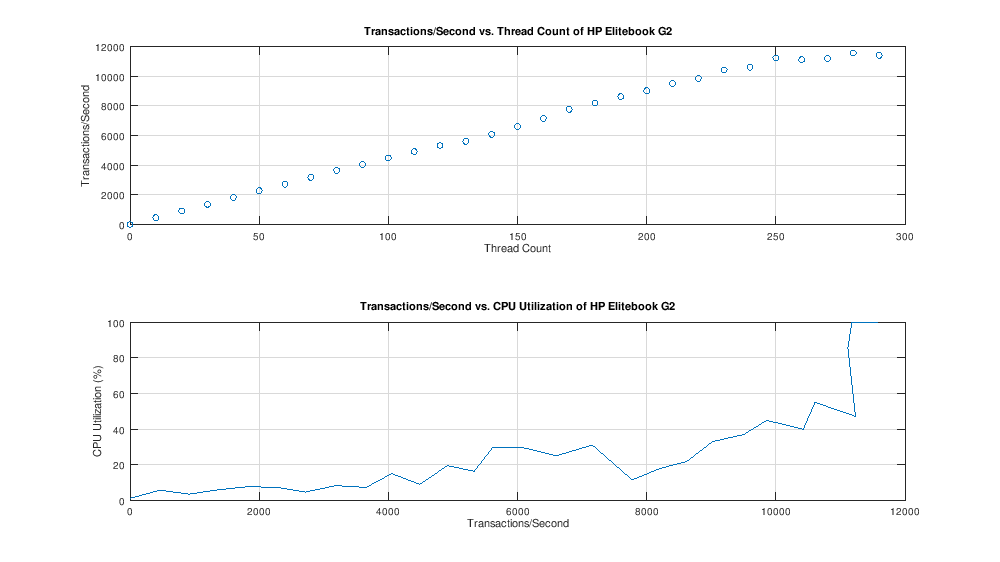
\includegraphics[width=5.75in]{bigGraph1.png}
	\caption{Computer Throughput Graphs}
	\label{fig1}
\end{figure}

\section*{Unnumbered Section}
This is section 3.

%\begin{thebibliography}{99}
% The numeral (here 99) in curly braces is nominally the number of entries in
% the bibliography. It's supposed to affect the amount of space around the
% numerical labels, so only the number of digits should matter--and even that
% seems to make no discernible difference.
%Not Requested
%\end{thebibliography}

\end{document}
